\chapter{Security and Privacy}

Software security is a high-priority concern for both product developers and users (since malicious attacks can cause losses to both). Figure \ref{fig:threats-security} shows the main types of security threats, even though there are some attacks that combine those threats (e.g., a ransomware attack threatening the integrity of system data also threatens system availability).

\begin{figure} [H]
    \centering
    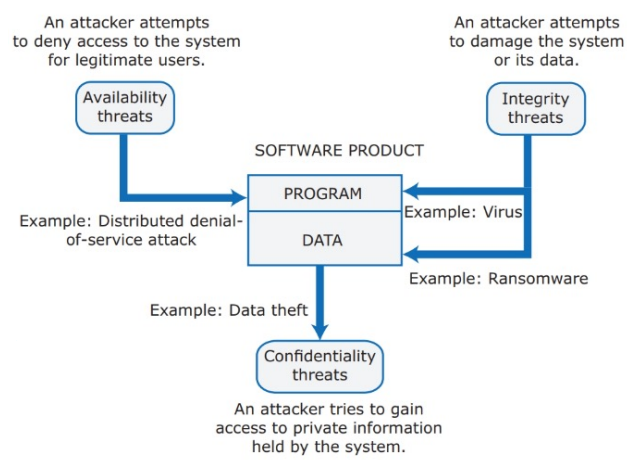
\includegraphics[width=0.8\textwidth]{images/Security/threats-security.png}
    \caption{Main types of security threats}
    \label{fig:threats-security}
\end{figure} 

Security is a \textbf{system-wide issue}: application software depends on the operating system, web server, language run-time system, database, frameworks, tools, and so on. Attacks may target any level of the system infrastructure stack, starting from the network.

\newpage
\noindent Some system management activities to maintain security are:
\begin{itemize}
    \item \textbf{Authentication and authorization standards and procedures} to ensure that all users have strong authentication and properly set up access permissions.
    \item \textbf{System infrastructure management} to keep infrastructure software properly configured and to promptly apply security updates patching vulnerabilities.
    \item Regularly \textbf{monitoring attacks} to promptly detect them and trigger resistance strategies to minimize the effects of an attack.
    \item \textbf{Backup policies} to keep undamaged copies of program and data files that can be restored after an attack.
\end{itemize}

\section{Attacks and defenses}

\subsection{Injection attacks}

An injection attack happens when a malicious user uses a valid input field to input malicious code or database commands to damage the system. One of the most common classes of attacks is \textbf{buffer overflow attacks}, which occur when an attacker can carefully craft an input string that includes executable instructions and overwrites memory. If a function return address is overwritten, control can be transferred to malicious code (e.g., on operating systems/libraries written in C/C++, which do not check whether array assignments are within array bounds).

Another common class of attacks is \textbf{SQL injection attacks}, which occur when an attacker can do an injection attack when user input is part of an SQL command. An easy countermeasure is to check input validity.

\subsection{Session hijacking attacks}

In many applications, there's the concept of a \textit{session}, which is a time period during which a user’s authentication with a web app is valid. This is usually achieved with session cookies (tokens) sent from the server to the client in each HTTP request, so the user doesn’t have to re-authenticate for subsequent system interactions (the session is closed when the user logs out or when the system “times out”).

Session hijacking is performed by an attacker who wants to acquire a valid session cookie in order to \textbf{impersonate a legitimate user}. An attacker can obtain the session cookie with a cross-site scripting attack or with traffic monitoring (which is easy on unsecured Wi-Fi networks and unencrypted data). The attack can either be \textbf{active} (the attacker carries out user actions on a server) or \textbf{passive} (the attacker simply monitors client-server traffic looking for valuable information, such as passwords, credit card numbers, and so on).

Some trivial defenses for this type of attack are to \textit{encrypt client-server network traffic} (using, for example, HTTPS), use \textit{multifactor authentication} to require confirmation of new actions that may be damaging, and use relatively \textit{short timeouts} on sessions.

\subsection{Cross-site scripting attacks}

Another form of injection attack is cross-site scripting attacks, where the attacker \textbf{adds malicious JavaScript code to the web page} returned from server to client. The malicious script is executed when the page is displayed in the victim’s browser, with the intention of stealing customer information or directing customers to another website (cookies may be stolen, making a session hijacking attack possible).

\begin{figure} [H]
    \centering
    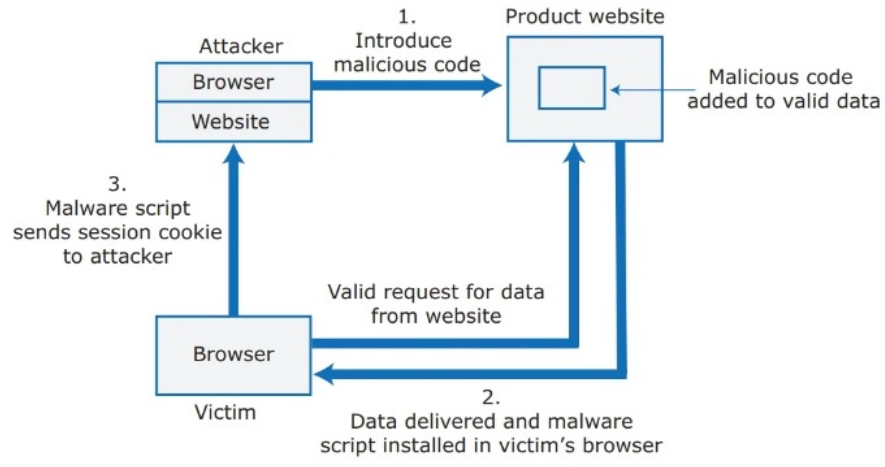
\includegraphics[width=0.93\textwidth]{images/Security/XSS.png}
    \caption{Cross-site scripting attack}
    \label{fig:XSS}
\end{figure} 

Some defenses for this kind of injection are (form) input validation, checking input from the database before adding it to the generated page, and employing the HTML “encode” command (info added to the web page is not executable).

\subsection{Denial-of-Service attacks}

Denial-of-Service attacks (DoS attacks) are intended to \textbf{make system unavailable} for normal use. This is usually performed with the usage of distributed computers (that have usually been hijacked) that are sending hundreds of thousands of requests for service to a web application. Those attacks aims to boycott server provider or to demand ransom payment. For this attack there are specialised software for detecting and dropping incoming packets, which helps to prevent the flooding of requests. More contermeasures are temporary user lockouts (e.g. lockout user by repeatedly failing authentication with user email address as login name), and IP address tracking (to restrict lockout when failed logins come from unusual IP addresses).

\subsection{Brute force attacks}

An attacker has only some information (e.g., a valid login name, but not the password) and repeatedly tries to guess the missing information. An attacker can use a string generator to \textbf{generate all possible combinations} of letters and numbers. The defenses for this type of attack are to convince (which means force) users to set long passwords that are not in a dictionary and are not common words. Another security layer can be added with the use of two-factor authentication.

\section{Authentication and Authorization}

\subsection{Authentication}

The objective of authentication is ensuring that users of your system are who they claim to be. Some approaches to achieve authentication are:
\begin{itemize}
    \item \textbf{Knowledge-based authentication} relies on users providing secret, personal information when registering. This type of authentication has weaknesses, such as \textit{insecure passwords}, \textit{phishing attacks} (users click on an email link pointing to a fake site that collects login and password), users using the \textit{same password}, and users regularly \textit{forgetting passwords} (a password recovery mechanism is needed, which means potential vulnerability if credentials have been stolen). Some ways to make this authentication method more secure are to force users to set strong passwords and to add personal questions for password recovery.

    \item \textbf{Possession-based authentication} relies on users having a physical device that can be linked to the authenticating system and that generates/displays information known to the authenticating system (e.g., the system sends a code to the user’s phone number or a special-purpose device that generates one-time codes).
    
    \item \textbf{Attribute-based authentication} relies on a unique biometric attribute of the user (e.g., fingerprint, face).
\end{itemize}

In cases where a system wants to store confidential user information, multi-factor authentication (e.g., password, then a code received on a mobile phone) is the best practice in order to add another layer of security.

Usually, developers don't implement authentication from scratch, but they use available toolkits and libraries (e.g., OAuth\footnote{\url{https://oauth.net/2/}}). Even when using already implemented libraries, there is still a lot of programming effort involved in order to implement a secure and reliable authentication system. This is why authentication systems are often outsourced with a \textbf{federated identity system}, which means using an external service for authentication (e.g., Google, Facebook, and so on), as shown in Figure \ref{fig:federated-identity}. These external services for authentication are proven to be secure and are likely to be much better than any independent system implemented by the product provider. On top of that, it allows the product provider to avoid maintaining their own database of passwords/secrets, as well as to gain additional user information (if the user agrees).

\begin{figure} [H]
    \centering
    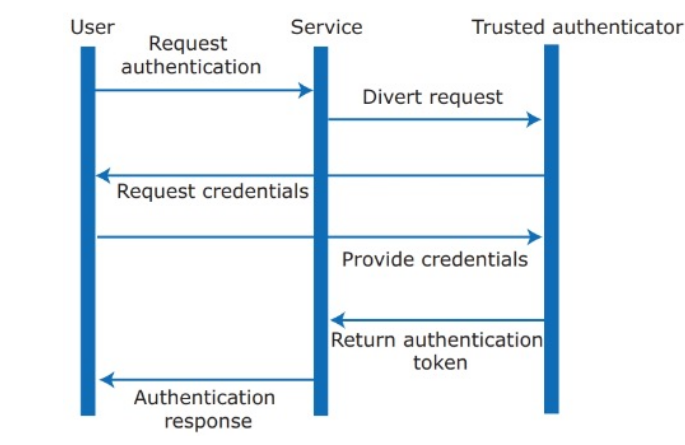
\includegraphics[width=0.85\textwidth]{images/Security/federated-identity.png}
    \caption{Federated identity sequence diagram}
    \label{fig:federated-identity}
\end{figure} 

\textbf{Mobile device authentication} plays by different rules, since usually typing passwords on mobile keyboards is inconvenient. An alternative to the written password could be to install an \textit{authentication token} on the mobile device, but this would lead to some weaknesses (if the device is stolen/lost, someone else can get access to the product). A safer alternative is to use \textit{individual users' digital certificates} (issued by trusted providers).

\subsection{Authorization}

While \textit{authentication} aims to ensure that the user is who they claim to be, \textit{authorization} wants to control that the user can access resources. It is required to have \textbf{access control} for multiuser products, where the access control policy \textit{must} reflect data protection rules that limit access to personal data (to prevent legal actions in case of a data breach).

One popular way to implement an access control policy is with \textbf{Access Control Lists} (ACLs): users are classified into groups (which dramatically reduces the size of ACLs), different groups can have different rights on different resources, and hierarchies of groups allow assigning rights to subgroups/individuals. We can see an example of an Access Control List in Figure \ref{fig:ACLs}.

\begin{figure} [H]
    \centering
    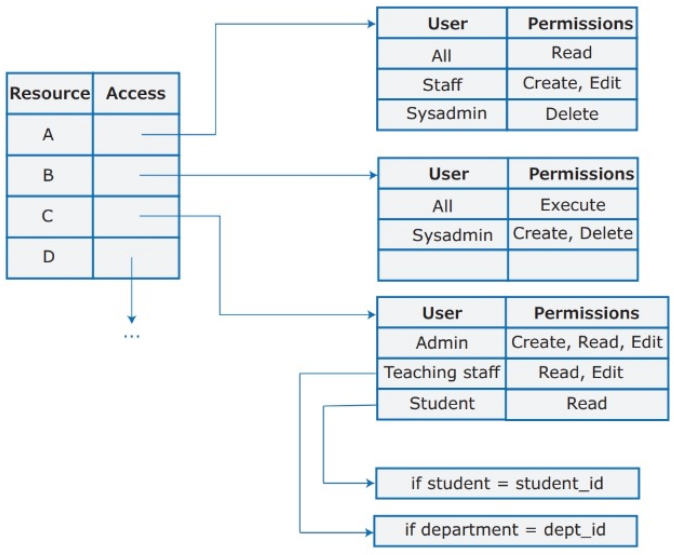
\includegraphics[width=0.85\textwidth]{images/Security/ACL.png}
    \caption{Example of Access Control Lists}
    \label{fig:ACLs}
\end{figure}

\section{Encryption}

\textit{Encryption} consists of making a text (typical data) unreadable by applying an algorithmic transformation to it. The text is encrypted with a secret key, travels through unsafe channels, and is then encrypted with the same or another key when it reaches its destination.

\textit{Modern encryption} techniques are considered “practically uncrackable” using currently available technology, even if history tells us that apparently uncrackable encryption may become crackable when new technology becomes available (what if/when quantum computers become commercially available one day?).

\noindent Usually, encryption is divided into two categories:

\begin{itemize}
    \item \textbf{Symmetric encryption}: older than the other method, used for centuries, but still used nowadays. Symmetric encryption uses the same key for encoding and decoding, but the sharing of the key is the weakness of this type of encryption.
    \item \textbf{Asymmetric encryption}: Asymmetric encryption uses different keys for encoding and decoding. This is the most secure encryption method, but also the most expensive one in terms of computation required for key generation. It's common practice to start the communication between two subjects using asymmetric encryption to share a symmetric key for the rest of the communication. 
\end{itemize}

\noindent\textbf{Transport Layer Security} (TLS) is a widely adopted security protocol designed to facilitate privacy and data security for communications over the Internet. A primary use case of TLS is encrypting the communication between web applications and servers, such as web browsers loading a website. This protocol can be built on top of the HTTP protocol, generating \textbf{HTTPS}, which is a standard practice for websites. TLS is also used to verify the identity of web servers with the use of \textbf{digital certificates} sent from servers to clients. Digital certificates are issued by trusted identity verification services (CAs). An example of a typical client-server handshake is shown in Figure \ref{fig:TLS}.

\begin{figure} [H]
    \centering
    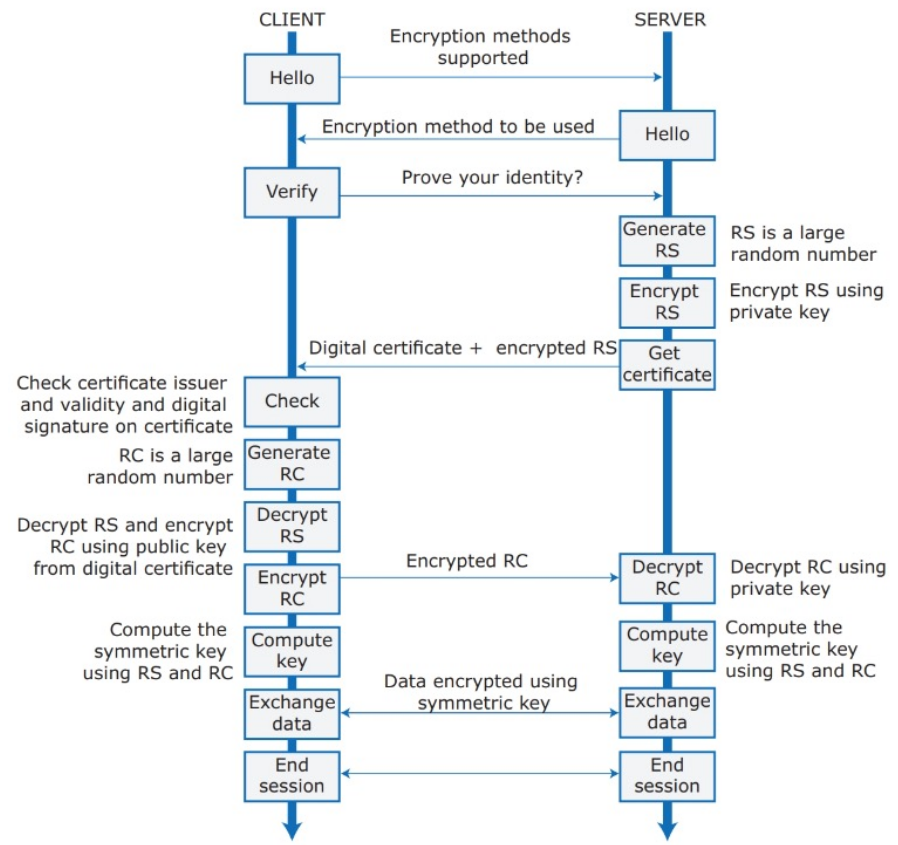
\includegraphics[width=0.8\textwidth]{images/Security/TLS.png}
    \caption{TLS client-server interaction to generate symmetric key for exchanging data}
    \label{fig:TLS}
\end{figure} 

\noindent It's interesting to understand when user data should be encrypted, and to do so we'll categorize data into:
\begin{itemize}
	\item \textbf{Data in transit} should always be encrypted since we want to achieve privacy in our communications.
	\item \textbf{Data at rest} (stored) should always be encrypted: in case of attacks, we don't want the attackers to obtain users' information in clear text.
	\item Encrypting and decrypting \textbf{data in use} (i.e., actively processed) slows down system response time.
\end{itemize}

\noindent Encryption of data is possible at four different levels in the system:
\begin{itemize}
	\item \textbf{Application level}: The application decides what data should be encrypted and decrypts that data immediately before it is used. This not only causes performance issues (security doesn't come for free), but it also requires some sort of key management. 
	\item \textbf{Database level}: The DBMS may encrypt the entire database when it's closed, with the database decrypted when it is reopened. Alternatively, individual tables or columns may be encrypted or decrypted.
	\item \textbf{Files level}: The operating system encrypts individual files when they are closed and decrypts them when they are reopened.
	\item \textbf{Media level}: The operating system encrypts disks when they are unmounted and decrypts these disks when they are remounted (useful for stolen/lost laptops).
\end{itemize}

All those levels require a key in order to encrypt and decrypt data. Data protection regulations may require that data copies are kept for years and stored securely, which means that if encryption keys get lost, encrypted data become permanently inaccessible! Keys should be changed periodically, and the database must maintain multiple timestamped versions of keys. To make life easier, \textbf{Key Management Systems} (KMS) are used to ensure that keys are securely generated, stored, and accessed by authorized users. Figure \ref{fig:KMS} shows how KMS are used.

\begin{figure} [H]
    \centering
    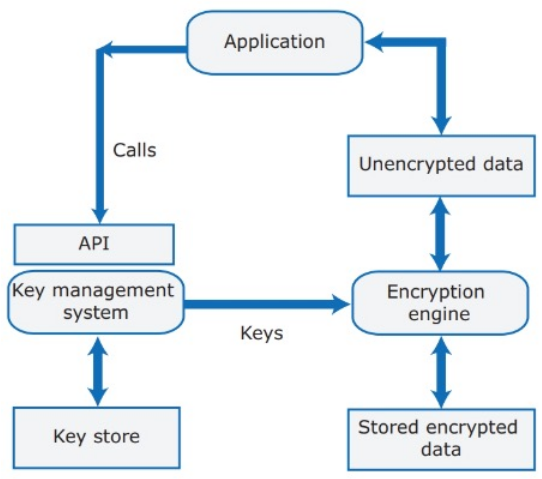
\includegraphics[width=0.7\textwidth]{images/Security/KMS.png}
    \caption{KMS usage schema}
    \label{fig:KMS}
\end{figure} 

\section{Privacy}

Privacy is a social concept that relates to the collection, dissemination, and appropriate use of personal information held by a third party.

\begin{figure} [H]
    \centering
    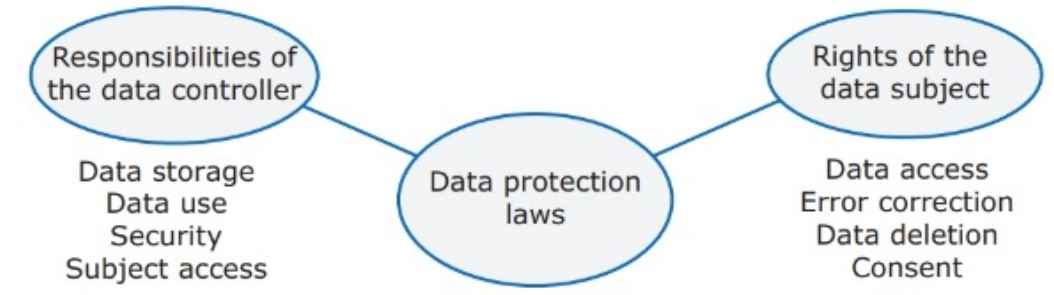
\includegraphics[width=0.9\textwidth]{images/Security/privacy-laws.png}
    \caption{Data protection laws}
    \label{fig:privacy-laws}
\end{figure} 

\noindent Some data protection principles are:
\begin{itemize}
    \item \textbf{Awareness and Control}: Users of your product must be made aware of what data is collected when they are using your product and must have control over the personal information that you collect from them.
    \item \textbf{Purpose}: You must tell users why data is being collected, and you must not use that data for other purposes.
    \item \textbf{Consent}: You must always have the consent of a user before you disclose their data to other people.
    \item \textbf{Data lifetime}: You must not keep data for longer than you need to. If a user deletes an account, you must delete the personal data associated with that account.
    \item \textbf{Secure storage}: You must maintain data securely so that it cannot be tampered with or disclosed to unauthorized people.
    \item \textbf{Discovery and error correction}: You must allow users to find out what personal data you store. You must provide a way for users to correct errors in their personal data.
    \item \textbf{Location}: You must not store data in countries where weaker data protection laws apply unless there is an explicit agreement that some stronger data protection rules will be upheld. 
\end{itemize}

\noindent There are also \textit{business reasons} for paying attention to information privacy:

\begin{itemize}
	\item If the system's conformance to privacy regulations does not match data protection regulations, the provider may be subject to legal actions or may not be able to sell their product.
	\item If a provider sells a business product, the provider's business customers may require privacy safeguards (not to be at risk with their users).
	\item Leakage or misuse of client information can damage the provider's reputation.
\end{itemize}

\noindent The information that software needs to collect depends on the functionality of the product and on the business model the provider uses. Here are more tips about data privacy:

\begin{itemize}
	\item Do not collect personal information that you do not need.
    \item Establish a privacy policy defining how personal/sensitive information about users is collected, stored, and managed.
	\item Make clear if you use users’ data to target advertising or to provide services that are paid for by other companies.
	\item If your product includes social network functionalities so that users can share information, you should ensure that users understand how to control the information they share.
\end{itemize}

\section{Security Smells}

\subsection{Challenges of Securing Microservices}

This subsection will outline the general properties of attacks and security specific to microservices. The illustration will be made with a list of key points:

\begin{itemize}
    \item \textit{The broader the attack surface, the higher the risk}: Since microservices trade data between each other using inter-service communication via remote calls, this means that (potentially) there are a large number of entry points, which \textbf{broadens the attack surface}. The security of the application depends on the weakest link: only one weak entry point can compromise the whole application.
    \item \textit{Distributed security screening affects performance}: Each microservice has to carry out independent security screening. This means that each service may need to connect to a remote security token service. Repeated, distributed security checks affect \textbf{performance}. A workaround for this problem is to \textit{trust the network} and skip security checks at each microservice, but a real solution (and also an industry trend) is to use \textit{zero-trust networking principles}, though overall performance must be considered.
    \newpage
    \item \textit{Bootstrapping trust among microservices needs automation}: Service-to-service communication must take place on protected channels. Suppose those services are using \textit{certificates}; each microservice must be provisioned with a certificate (and corresponding private key) to authenticate itself to another microservice during service-to-service interactions. The receiver must know how to validate the certificate of the calling microservice, so there is a need to \textbf{bootstrap trust} between microservices (including the need to revoke and rotate certificates). To manage large-scale deployments of hundreds of microservices, \textit{automation} is needed.
    \item \textit{Tracing requests spanning multiple microservices is challenging}: Logs can be aggregated to produce \textit{metrics} that reflect system state (e.g., average invalid access requests per hour) and may trigger alerts. Traces help track a request from the point where it enters the system to the point where it leaves. Unlike monolithic applications, a request in a microservices deployment may span multiple microservices, making \textbf{correlating requests among microservices challenging}.
    \item \textit{Containers complicate credentials/policies handling}: Containers are \textit{immutable servers} (great for simplifying deployment and achieving horizontal scalability), so they don’t change state after spin-up. Since each service needs to maintain a dynamic list of allowed clients and a dynamic set of access-control policies, the only way to modify these lists periodically is to keep credentials in the container filesystem and \textbf{inject them at boot time}.
    \item \textit{Distribution makes sharing user context harder}: When a request starts to move inside the system, there is a lot of information we want to associate with the request (e.g., whether it’s a premium or non-premium request). The challenge is to \textit{build trust between microservices} so that the receiving microservice accepts the user context passed from the calling microservice (a security attack can occur if user information is manipulated). A popular solution is \textbf{JSON Web Token} (JWT), a security token used to share user context among microservices.
    \item \textit{Security responsibilities distributed among different teams}: Different independent teams can use \textbf{different technology stacks} (such as security best practices and various tools for static and dynamic security testing). Security responsibilities are distributed across different teams. Organizations often adopt a hybrid approach with a centralized security team and security experts within the teams.
\end{itemize}
\newpage
\subsection{Smells and Refactoring}

A \textbf{security smell} is a commonly used architectural decision that indicates possible security violations in microservice-based applications. Once the microservice principles are defined, how can \textcolor{red}{security smells} that affect \textcolor{blue}{security properties} of microservices be detected and resolved via \textcolor{green}{refactoring}?

This section will show, based on a \textit{multivocal review} (which uses both scientific articles and technical websites), which are the most recognized \textit{security smells} for microservices and the security \textit{refactorings} to resolve them. 

\noindent The \textbf{security properties} that will be considered are:

\begin{itemize}
    \item \textcolor{blue}{Confidentiality}: The degree to which a product or system ensures that data is accessible only to those authorized to have access.
    \item \textcolor{blue}{Integrity}: The degree to which a system, product, or component prevents unauthorized modification of computer programs or data.
    \item \textcolor{blue}{Authenticity}: The degree to which the identity of a subject or resource can be proven to be the one claimed.
\end{itemize}

\noindent Since some \textit{security smells} violate multiple \textit{security properties}, the following list will show all the \textcolor{red}{security smells}, their related \textcolor{blue}{security properties}, and how to \textcolor{green}{refactor} them:

\begin{itemize}
    \item \textcolor{red}{Insufficient access control}: Some services of an application don't implement access control, leading to a \textit{confused deputy problem} (an attacker obtaining data they shouldn’t access), causing potential violations of the \textcolor{blue}{confidentiality} of data (and business functions). Client permissions need to be verified at request time without introducing extra latency and contention with frequent calls to a centralized service. One way to refactor this smell is to \textcolor{green}{use OAuth 2.0}, a token-based security framework for delegated access control.
    \item \textcolor{red}{Publicly accessible microservices}: Some microservices are directly accessible by external clients. Each such microservice must check authentication and authorization for each request (increasing the cost of application maintenance), but this also increases the exposure of credentials, which could lead to \textcolor{blue}{confidentiality} violations. The most cited refactoring is the \textcolor{green}{implementation of an API gateway}, which can (from behind a firewall) enforce authentication, authorization, throttling, and message content validation.
    \item \textcolor{red}{Unnecessary privileges to microservices}: Sometimes microservices are granted unnecessary access levels, permissions, or functionalities that are not needed to deliver their business functions. This mostly arises because programmers copy and paste similar patterns, leading to unnecessary access. When resources are unnecessarily exposed, the attack surface against \textcolor{blue}{confidentiality} and \textcolor{blue}{integrity} is increased. The refactoring is to \textcolor{green}{follow the Least Privilege Principle.} \footnote{\textbf{Least Privilege Principle}: \textit{Allow running code only the permissions needed to complete the required tasks and no more}.}
    \item \textcolor{red}{``Home-made'' crypto code}: The usage of ``home-made'' cryptography code can cause \textcolor{blue}{confidentiality}, \textcolor{blue}{integrity}, and \textcolor{blue}{authenticity} issues, which can be worse than no encryption at all (because of the false sense of security). The solution is to \textcolor{green}{use encryption libraries that are heavily tested} by the community and regularly reviewed and patched (avoid experimental encryption algorithms).
    \item \textcolor{red}{Non-encrypted data exposure}: A microservice-based application accidentally exposes sensitive data (e.g., data stored without encryption or protection that has vulnerabilities), allowing intruders to access or modify data, including credentials, leading to violations of \textcolor{blue}{confidentiality}, \textcolor{blue}{integrity}, and \textcolor{blue}{authenticity}. The refactor is to \textcolor{green}{encrypt all sensitive data at rest}: All sensitive data should always remain encrypted and only be decrypted when needed. Most DBMSs support automatic encryption, but encryption can also be applied at the application level, OS level, and cache level. It's important to note that encryption is resource-consuming, so critical data should be identified, and encryption should be applied only when needed.
    \item \textcolor{red}{Hardcoded secrets}: Hardcoded secrets (e.g., API keys, client secrets, credentials) should never be stored in environment variables because they could be accidentally exposed (e.g., exception handlers may send info to a logging platform), leading to violations of \textcolor{blue}{confidentiality}, \textcolor{blue}{authenticity}, and \textcolor{blue}{integrity}. The solution is to \textcolor{green}{encrypt secrets at rest}, avoid storing credentials alongside applications or in source code repositories, and refrain from using environment variables to pass secrets.
    \item \textcolor{red}{Non-secured service-to-service communications}: Microservices interacting without secure communication channels could expose data to man-in-the-middle, eavesdropping, and tampering attacks, leading to potential violations of \textcolor{blue}{confidentiality}, \textcolor{blue}{integrity}, and \textcolor{blue}{authenticity}. A widely accepted solution is to \textcolor{green}{use mutual Transport Layer Security}, which encrypts data in transit and ensures its integrity and confidentiality. Mutual TLS also allows a microservice to legitimately identify the microservice it is communicating with (\textit{mutual authentication}).
    \item \textcolor{red}{Unauthenticated traffic}: It's crucial that microservices authenticate one another (especially when user context is passed). If traffic is not authenticated, microservices are exposed to security attacks like data tampering, denial of service, or privilege elevation, leading to \textcolor{blue}{authenticity} issues. As mentioned before, \textcolor{green}{Transport Layer Security} allows mutual authentication. It's also possible to use \textcolor{green}{OpenID Connect}, which uses JWT containing authenticated user information, where microservices verify user identity with authorization servers.
    \item \textcolor{red}{Multiple user authentication}: As software engineers, it's tempting to make users authenticate from different points. Each access point constitutes a potential attack vector for intruders to authenticate as end users, leading to \textcolor{blue}{authenticity} issues. The most suggested approach is to use \textcolor{green}{Single Sign-On} (single entry point), which facilitates log storage and auditing. Single sign-on can be achieved by employing an \textcolor{green}{API gateway} and \textcolor{green}{OpenID Connect} (to share user contexts).
    \item \textcolor{red}{Centralized authorization}: Authorization can be enforced at the edge of the application (API gateway) and/or by each microservice. If authorization is only handled at the edge, the “central” authorization point becomes a bottleneck, reducing performance and efficiency. There is also the possibility of a “confused deputy problem“: microservices trust the gateway based on its mere identity, leading to potential violations of \textcolor{blue}{authenticity}. The solution is to enact a \textcolor{green}{decentralized authorization approach} by transmitting an access token (e.g., JWT) together with each request to a microservice and granting access to the caller only if a known token is passed.
\end{itemize}

\subsection{Refactor or Not Refactor?}

This question should be addressed on a case-by-case basis: \textbf{solving a smell may affect other properties}! For example, centralized and decentralized authorization: while switching to decentralized authorization follows certain declared \textit{design principles} and ensures \textit{security properties}, centralized authorization is easier to \textit{maintain} and offers \textit{better performance}.

Modeling soft goal interdependencies as \textbf{graphs} can help with visualization and (automated) trade-off analysis. An example is shown in Figure \ref{fig:authorization}.

\begin{figure} [H]
    \centering
    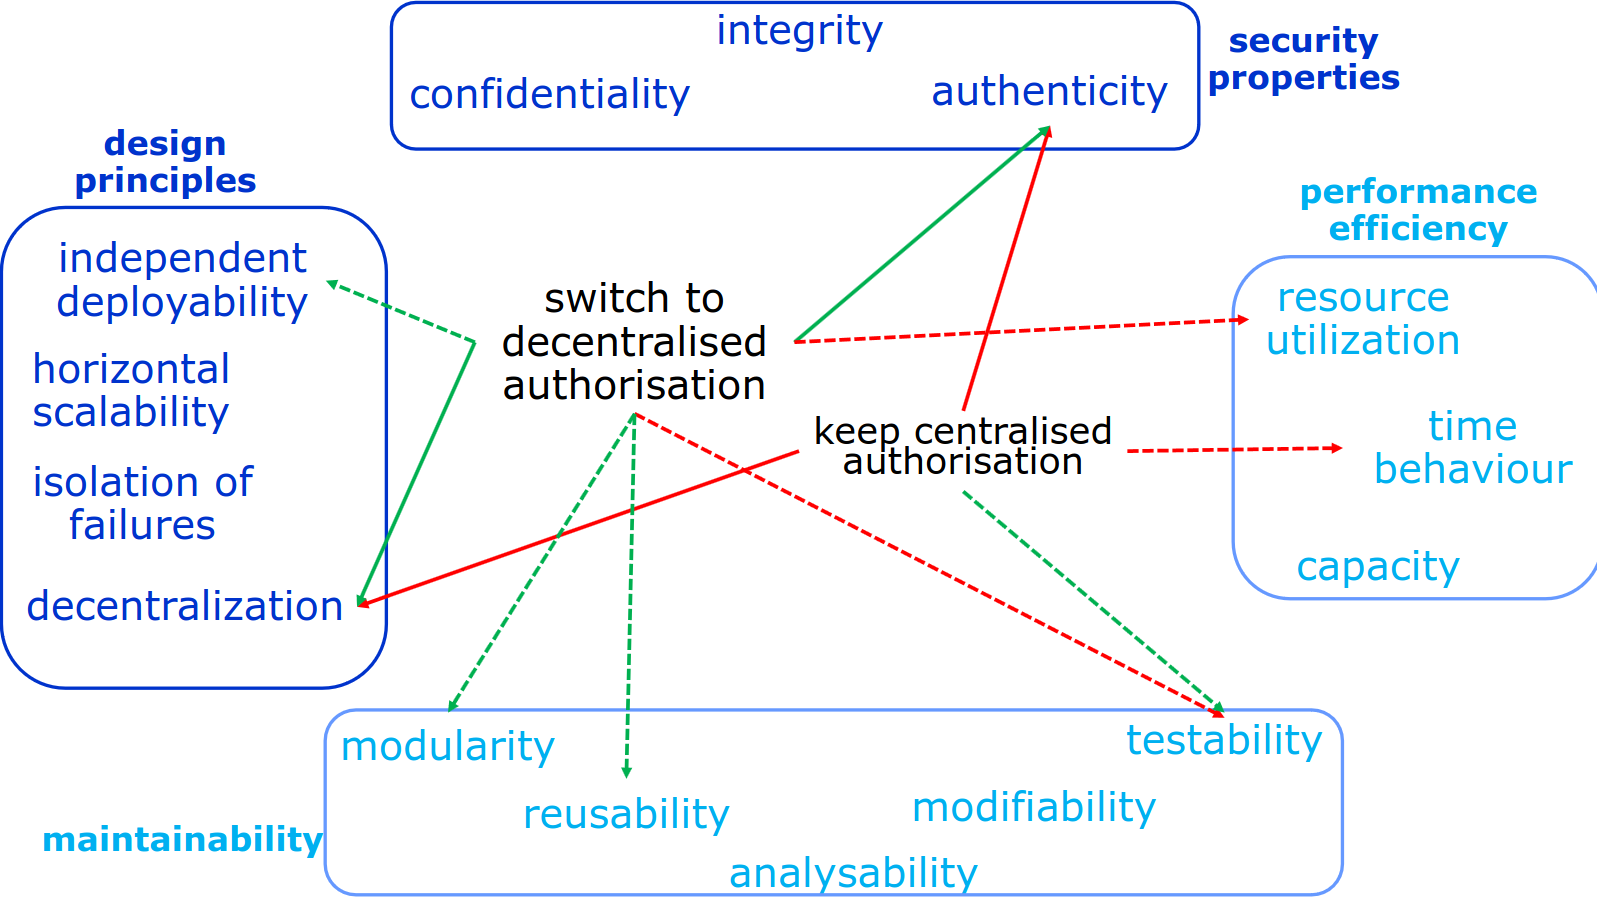
\includegraphics[width=0.79\textwidth]{images/Security/authorization.png}
    \caption{Comparison between centralized authorization and decentralized authorization}
    \label{fig:authorization}
\end{figure}
